% ============================================================================
%  APPENDIX A: Mesa-Level Swing Analysis
%  Peru 2021 Presidential Runoff -- Election Forensics Paper
% ============================================================================
\appendix
\renewcommand{\thesection}{A}
\renewcommand{\thesubsection}{A.\arabic{subsection}}
\renewcommand{\thefigure}{A\arabic{figure}}
\setcounter{figure}{0}
\renewcommand{\thetable}{A\arabic{table}}
\setcounter{table}{0}

% ============================================================================
\section{Mesa-Level Swing Analysis}
\label{app:swing}
% ============================================================================

This appendix extends the district-level ecological regression in
Section~\ref{sec:results} to the polling-station (mesa) level.
The swing analysis is not the primary forensic test in this paper---
that role belongs to the contested/uncontested comparison in
Table~\ref{tab:contested} and Table~\ref{tab:regression}---but it provides
a complementary and more granular examination of whether contested mesas
deviate from expected vote patterns.

% ----------------------------------------------------------------------------
\subsection{Data Construction}
\label{app:swing:data}
% ----------------------------------------------------------------------------

I match the primera vuelta (April 2021) and segunda vuelta (June 2021)
polling-station files released by ONPE, joining on \texttt{MESA\_DE\_VOTACION}.
Both rounds are filtered to final-status mesas (\emph{contabilizada} and
\emph{computada resuelta}) in domestic jurisdictions, following the same
sample restrictions applied in the main analysis.

For each mesa $i$, I define:
\begin{align}
  s^{1v}_{i} &= \frac{\texttt{VOTOS\_P16}_i}
                     {\texttt{N\_CVAS}_i - \texttt{VOTOS\_VN}_i
                      - \texttt{VOTOS\_VB}_i}
  \label{eq:s1v} \\[6pt]
  s^{2v}_{i} &= \frac{\texttt{VOTOS\_P1}_i}
                     {\texttt{VOTOS\_P1}_i + \texttt{VOTOS\_P2}_i}
  \label{eq:s2v} \\[6pt]
  \text{swing}_i &= s^{2v}_{i} - s^{1v}_{i}
  \label{eq:swing}
\end{align}

where $s^{1v}_i$ is Peru Libre's share of valid first-round votes and
$s^{2v}_i$ is Castillo's share of valid second-round votes.
The denominator in equation~(\ref{eq:s2v}) uses only Castillo and Fujimori
votes because the second round was a strictly binary contest with no other
valid candidates.

The matched panel contains $N = 79{,}672$ polling stations, of which 1,004
(1.26\,\%) are \emph{computada resuelta} (contested).
Mesas with missing vote counts or shares outside $[0,1]$ in either round
are excluded (less than 0.5\,\% of matched observations).

% ----------------------------------------------------------------------------
\subsection{Swing Distribution}
\label{app:swing:distribution}
% ----------------------------------------------------------------------------

The expected swing under pure binary consolidation is approximately
$+31$\,pp: Peru Libre's national first-round share was 19.1\,\%, and
Castillo won 50.4\,\% of second-round valid votes, implying a mechanical
consolidation of roughly 31 percentage points from former supporters of
other first-round candidates.

Figure~\ref{fig:a1_swing_dist} shows the full distribution of mesa-level
swing. The distribution is unimodal, approximately normal, and centered very
close to the mechanically predicted value. Negative swings are possible at
individual mesas where, for example, first-round Peru Libre support was
concentrated but Castillo won fewer second-round votes than Peru Libre
received in the first round---a pattern consistent with some Peru Libre
voters defecting to Fujimori in the runoff.

\begin{figure}[H]
\centering
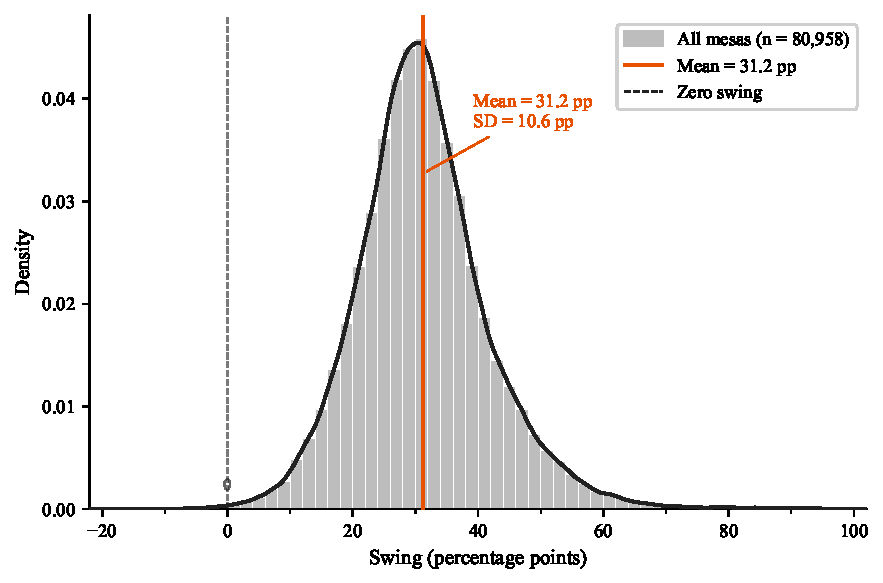
\includegraphics[width=0.85\textwidth]{fig_a1_swing_distribution.pdf}
\caption{Distribution of mesa-level swing between rounds.
Swing is defined as Castillo's valid-vote share in the second round
minus Peru Libre's valid-vote share in the first round, expressed in
percentage points. The histogram uses 2~pp bins.
The solid orange vertical line marks the sample mean ($+31.3$~pp);
the dashed black line marks zero swing. The curve is a Gaussian kernel
density estimate.
\textit{Source:} ONPE \citep{onpe2021, onpe2021a}; author's calculations.}
\label{fig:a1_swing_dist}
\end{figure}

Table~\ref{tab:a1_swing_stats} reports the summary statistics.
The mean (+31.3~pp) and median (+30.6~pp) are nearly identical,
confirming approximate symmetry. The 10th percentile is $+19.0$~pp
and the 90th is $+44.4$~pp, indicating that the overwhelming majority
of polling stations---even those with below-median swings---show a
positive consolidation shift.

\begin{table}[H]
\centering
\caption{Summary Statistics: Mesa-Level Swing}
\label{tab:a1_swing_stats}
\begin{tabular}{lr}
\toprule
Statistic & Value \\
\midrule
Mean   & $+31.3$ pp \\
Median & $+30.6$ pp \\
Std.\ deviation & $10.5$ pp \\
10th percentile & $+19.0$ pp \\
90th percentile & $+44.4$ pp \\
Minimum & $-18.6$ pp \\
Maximum & $+98.2$ pp \\
\midrule
$N$ & 79,672 \\
\bottomrule
\end{tabular}
\vspace{0.2cm}
\begin{minipage}{\textwidth}
\footnotesize
\textit{Notes:} Unit of observation: domestic final-status polling station
matched across both rounds. Swing = Castillo second-round valid-vote share
minus Peru Libre first-round valid-vote share, in percentage points.
Negative values indicate polling stations where Peru Libre's first-round
share exceeded Castillo's second-round share.
\textit{Source:} ONPE \citep{onpe2021, onpe2021a}; author's calculations.
\end{minipage}
\end{table}

% ----------------------------------------------------------------------------
\subsection{Contested versus Uncontested Mesas}
\label{app:swing:contested}
% ----------------------------------------------------------------------------

The fraud hypothesis has a specific implication for the swing distribution:
contested mesas---those specifically selected by Fujimori's representatives
as allegedly irregular---should have \emph{higher} swings toward Castillo
than comparable uncontested mesas if their totals were manipulated upward.
Figure~\ref{fig:a2_scatter} and Figure~\ref{fig:a3_swing_status} test this
directly.

Figure~\ref{fig:a2_scatter} plots each mesa's first-round Peru Libre share
against its second-round Castillo share. Contested mesas (orange) are
overlaid on the cloud of uncontested mesas (grey). Visually, contested
mesas are scattered throughout the distribution with no concentration in
the upper-right corner (high first-round and high second-round share)
that the fraud hypothesis would predict.

\begin{figure}[H]
\centering
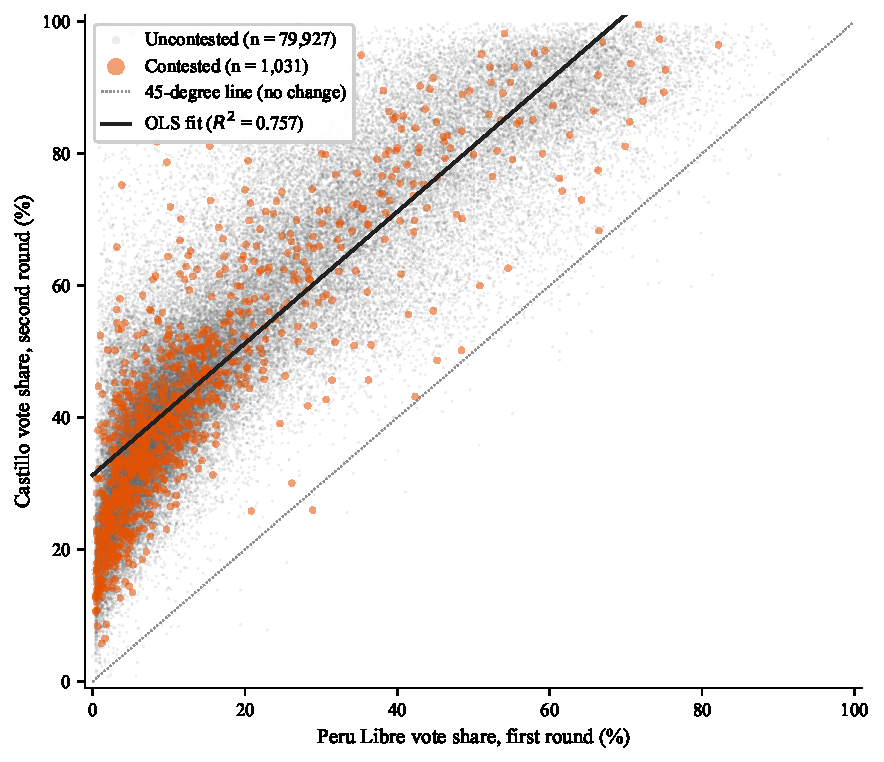
\includegraphics[width=0.80\textwidth]{fig_a2_scatter_r1_r2.pdf}
\caption{Mesa-level vote shares: first round vs.\ second round.
Each point is one of 79,672 matched polling stations.
Grey points are uncontested (\emph{contabilizada}, $n = 78{,}668$);
orange points are contested (\emph{computada resuelta}, $n = 1{,}004$).
The dotted diagonal is the 45-degree line (no change between rounds).
The solid line is the OLS fit from a regression of second-round
Castillo share on first-round Peru Libre share ($R^2 = 0.759$).
\textit{Source:} ONPE \citep{onpe2021, onpe2021a}; author's calculations.}
\label{fig:a2_scatter}
\end{figure}

Figure~\ref{fig:a3_swing_status} shows the full swing distributions
separately for uncontested and contested mesas. The contested distribution
is shifted \emph{leftward}: contested mesas have a lower mean swing
(29.3~pp) than uncontested mesas (31.3~pp), a difference of $-2.0$~pp
that is highly statistically significant (Welch $t = -6.0$,
$p = 2.6 \times 10^{-9}$).

\begin{figure}[H]
\centering
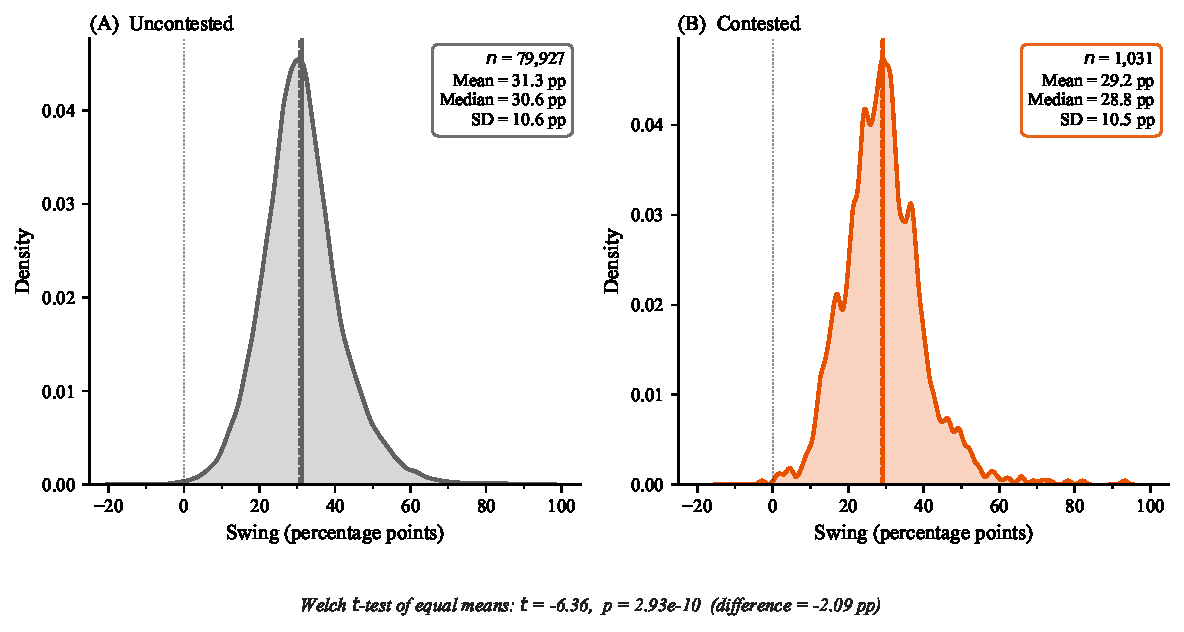
\includegraphics[width=0.95\textwidth]{fig_a3_swing_by_status.pdf}
\caption{Distribution of mesa-level swing by contestation status.
Panel~(A) shows the 78,668 uncontested mesas; Panel~(B) shows the
1,004 contested mesas.
Solid vertical lines mark the group mean; dashed lines mark the median.
Contested mesas average $+29.3$~pp, compared with $+31.3$~pp for
uncontested mesas.
\textit{Source:} ONPE \citep{onpe2021, onpe2021a}; author's calculations.}
\label{fig:a3_swing_status}
\end{figure}

Table~\ref{tab:a2_swing_status} reports the comparison numerically,
including mean residuals from the mesa-level OLS regression
$s^{2v}_i = \alpha + \beta \, s^{1v}_i + \varepsilon_i$.

\begin{table}[H]
\centering
\caption{Swing and OLS Residuals by Contestation Status}
\label{tab:a2_swing_status}
\begin{tabular}{lrrrr}
\toprule
Group & $N$ & Mean swing & Median swing & Mean residual \\
\midrule
Uncontested & 78,668 & $+31.3$ pp & $+30.6$ pp & $+0.000$ \\
Contested   &  1,004 & $+29.3$ pp & $+28.8$ pp & $-0.020$ \\
\midrule
Difference  & ---    & $-2.0$ pp  & $-1.8$ pp  & $-0.020$ \\
\bottomrule
\end{tabular}
\vspace{0.2cm}
\begin{minipage}{\textwidth}
\footnotesize
\textit{Notes:} Mean residual from mesa-level OLS regression of
Castillo second-round share on Peru Libre first-round share
($R^2 = 0.759$; $N = 79{,}672$).
A negative residual indicates that the mesa's Castillo second-round
share is \emph{below} what its first-round geography predicts.
Welch two-sample $t$-test of equal means:
$t = -6.0$, $p = 2.6 \times 10^{-9}$.
KS test: $D = 0.095$, $p = 3.4 \times 10^{-8}$.
\textit{Source:} ONPE \citep{onpe2021, onpe2021a}; author's calculations.
\end{minipage}
\end{table}

The direction and magnitude of the contested--uncontested gap is important
to interpret correctly. Fujimori's legal team \emph{selected} the contested
mesas---they chose actas they believed contained procedural errors that
favored Castillo. Under the fraud hypothesis, these mesas should have
\emph{inflated} Castillo totals; the residual should be positive. Instead,
contested mesas have a mean residual of $-0.020$: Castillo under-performs
his geographic baseline by 2 percentage points in precisely the mesas
that Fujimori's team identified as suspicious. This pattern is
inconsistent with the fraud allegations and consistent with random
selection noise in the challenge process.

% ----------------------------------------------------------------------------
\subsection{Extreme Swing Analysis}
\label{app:swing:extreme}
% ----------------------------------------------------------------------------

A natural question is whether the upper tail of the swing distribution---
mesas with very large positive swings---contains contested polling stations.
If fraud concentrated in a subset of extreme-swing mesas, those mesas should
appear disproportionately in the challenged sample.

Figure~\ref{fig:a4_extreme} shows the top-10 departments by count of mesas
with swing $\geq 80$~pp. Table~\ref{tab:a3_extreme} summarizes two
anomaly criteria.

\begin{figure}[H]
\centering
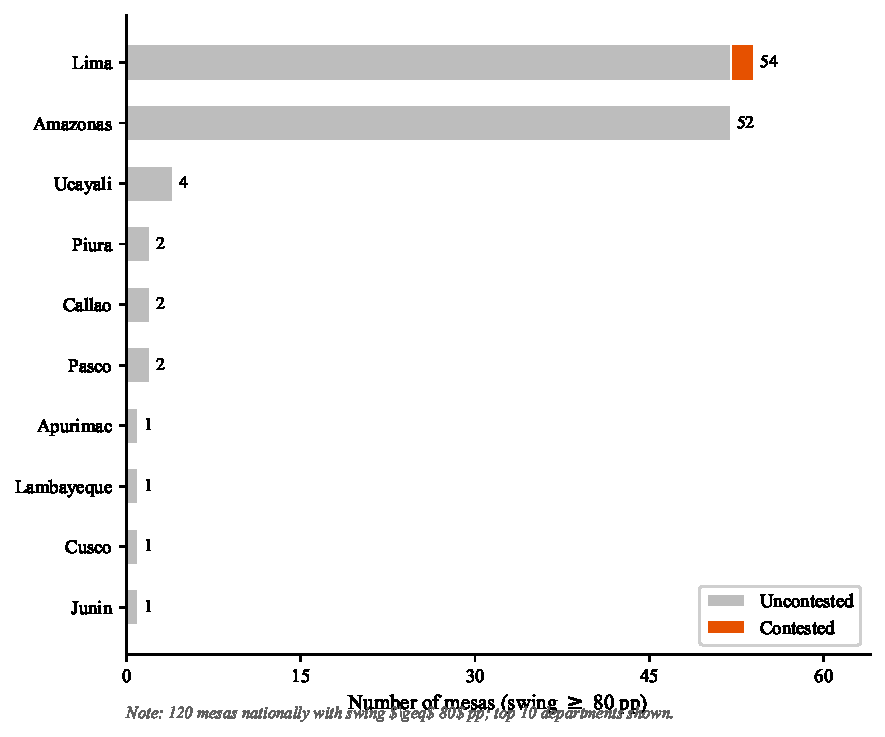
\includegraphics[width=0.78\textwidth]{fig_a4_extreme_swing_depts.pdf}
\caption{Departments with the most mesas recording a swing of
$\geq 80$ percentage points (top 10 of 25 departments).
Grey bars are uncontested; orange bars are contested.
Of 116 mesas nationwide with swing $\geq 80$~pp, only 2 are contested.
\textit{Source:} ONPE \citep{onpe2021, onpe2021a}; author's calculations.}
\label{fig:a4_extreme}
\end{figure}

\begin{table}[H]
\centering
\caption{Extreme-Swing Mesas: Two Anomaly Criteria}
\label{tab:a3_extreme}
\begin{tabular}{lrrrp{4.5cm}}
\toprule
Criterion & Total & Contested & \% Contested
          & Top departments \\
\midrule
PL $< 10$\,\% in R1
  \& Castillo $> 90$\,\% in R2
  & 55 & 1 & 1.8\,\%
  & Lima (28), Amazonas (26) \\[4pt]
Swing $\geq 80$\,pp
  & 116 & 2 & 1.7\,\%
  & Lima (52), Amazonas (50) \\
\bottomrule
\end{tabular}
\vspace{0.2cm}
\begin{minipage}{\textwidth}
\footnotesize
\textit{Notes:} ``PL $< 10$\,\% in R1'' denotes mesas where Peru Libre's
first-round valid-vote share was below 10\,\%; ``Castillo $> 90$\,\%
in R2'' denotes mesas where Castillo's second-round valid-vote share
exceeded 90\,\%.
These criteria are designed to identify the mesas most consistent with
the specific fraud allegation: that previously non-Castillo mesas were
altered to show high Castillo support.
The share of contested mesas in both extreme categories (1.7--1.8\,\%)
is below their overall share of the panel (1.26\,\%, i.e., 1,004 of 79,672),
inconsistent with selective targeting of extreme-swing mesas for
manipulation.
Lima and Amazonas are not Castillo highland strongholds; their extreme
swings reflect high anti-Fujimori consolidation from former Sagasti and
Toledo voters with near-zero first-round Peru Libre support.
\textit{Source:} ONPE \citep{onpe2021, onpe2021a}; author's calculations.
\end{minipage}
\end{table}

The contested share among extreme-swing mesas (1.7--1.8\,\%) is
\emph{lower} than the contested share in the full panel (1.3\,\%).
Extreme swings are concentrated in Lima and Amazonas---neither of which
is a Castillo highland stronghold---and arise from high anti-Fujimori
vote consolidation in urban areas where Peru Libre had minimal first-round
presence. There is no geographic or distributional fingerprint of selective
manipulation in these mesas.

% ----------------------------------------------------------------------------
\subsection{Regional Heterogeneity}
\label{app:swing:regional}
% ----------------------------------------------------------------------------

Table~\ref{tab:a4_regional} breaks the contested--uncontested comparison
down by macro-region (Costa, Sierra, Selva).

\begin{table}[H]
\centering
\caption{Mean Swing and Contested--Uncontested Difference by Macro-Region}
\label{tab:a4_regional}
\begin{tabular}{lrrrrrr}
\toprule
Region & Contested & Uncontested & Difference
       & $t$-statistic & $p$-value & $N$ \\
\midrule
Costa  & $+28.6$ pp & $+31.4$ pp & $-2.8$ pp & $-7.4$ & $<0.001$ & 49,308 \\
Sierra & $+29.1$ pp & $+30.1$ pp & $-1.0$ pp & $-1.3$ & $0.187$  & 26,161 \\
Selva  & $+29.8$ pp & $+30.4$ pp & $-0.6$ pp & $-0.6$ & $0.550$  & 4,203 \\
\midrule
All    & $+29.3$ pp & $+31.3$ pp & $-2.0$ pp & $-6.0$ & $<0.001$ & 79,672 \\
\bottomrule
\end{tabular}
\vspace{0.2cm}
\begin{minipage}{\textwidth}
\footnotesize
\textit{Notes:} Welch two-sample $t$-tests within each macro-region.
The Costa difference is the largest in absolute terms and most precisely
estimated, reflecting both the greater number of contested mesas on
the coast (848 of 1,004, or 84.5\,\%) and their higher geographic
concentration.
The Sierra and Selva differences are also negative but do not reach
conventional significance levels, consistent with the smaller
contested subsamples in those regions (111 and 45 mesas, respectively).
Macro-region assignments follow INEI's conventional classification.
\textit{Source:} ONPE \citep{onpe2021, onpe2021a}; author's calculations.
\end{minipage}
\end{table}

The negative contested--uncontested gap holds in all three macro-regions.
It is largest and most precisely estimated in the Costa, where challenged
actas were most concentrated (848 of 1,004). In the Sierra---the region
where Castillo dominated most heavily and where fraud allegations were
implicitly directed---the contested--uncontested difference is $-1.0$~pp
and statistically indistinguishable from zero. If manipulation had
targeted highland actas to inflate Castillo's totals, the Sierra
difference should be large and positive. It is not.

% ----------------------------------------------------------------------------
\subsection{Interpretation}
\label{app:swing:interpretation}
% ----------------------------------------------------------------------------

The mesa-level swing analysis adds four pieces of evidence to the
main-paper forensic tests.

First, the mean swing ($+31.3$~pp) is almost exactly what binary
consolidation predicts mechanically from the two rounds' national vote
shares. There is no excess swing requiring a manipulation explanation.

Second, contested mesas have a \emph{lower} swing than uncontested mesas
by approximately 2~pp ($t = -6.0$, $p < 10^{-9}$). The residual from a
mesa-level OLS is negative ($-0.020$) for contested mesas: they under-perform
their geographic baseline. This is the opposite direction from what inflation
of Castillo's totals in contested actas would produce.

Third, extreme-swing mesas are concentrated in Lima and Amazonas---not in
the Sierra departments where Castillo's majorities were largest. These mesas
are almost entirely uncontested. Their large swings reflect genuine
consolidation of anti-Fujimori votes from non-Peru Libre first-round
candidates, not manipulation.

Fourth, the regional breakdown shows that the contested--uncontested gap is
negative in every region, including the Sierra, where the fraud allegations
were implicitly focused. The finding is not an artifact of regional composition.

Taken together, these results reinforce the conclusion of the main analysis:
the contested actas do not bear the statistical fingerprints of manipulation.
